\section{Auswertung}
\label{sec:Auswertung}

Im Folgenden wird die Auswertung der verschiedenen Messungen präsentiert. Die Fehlerrechnungen und Ausgleichsrechnungen werden mittels \textit{Python} durchgeführt.
Für die verwendeten physikalischen Konstanten wurde die \textit{Python}-Bibliothek \textit{SciPy} \cite{scipy} verwendet.

\subsection{Magnetfeldmessung}

Die Eichung des Elektromagneten erfolgt \"uber eine Ausgleichsrechnung an die Messdaten des Magnetfeldes.
Daf\"ur wird eine Polynomgleichung dritten Gerades an die Hysteresekurve gefittet.
\begin{align}
  B(x) = A x^3 + B x^2 + C x + D
\end{align}
In Tabelle \ref{tab:magnetfeld} sind die ermittelten Parameter der Ausgleichsrechnung f\"ur die zwei aufsteigenden
und die abfallende Hysteresekurve. 
\begin{table}
  \centering
  \begin{tabular}{c c c c}
    \toprule
    $A$ / mT/$\symup{A^3}$ & $B$ / mT/$\symup{A^2}$ & $C$ / mT/$\symup{A}$ & $D$ / mT\\
    \midrule
        \SI{-0.26(5)}{}  &  \SI{7(2)}{}   &  \SI{10(13)}{}   & \SI{30(33)}{}  \\
        \SI{-0.10(2)}{}  &  \SI{2.1(7)}{}  &  \SI{48(6)}{}   & \SI{11(14)}{}  \\
        \SI{-0.09(2)}{}  &  \SI{2.3(8)}{}  &  \SI{43(7)}{}   & \SI{32(16)}{}  \\
    \bottomrule
  \end{tabular}
  \caption{Ermittelte Parameter der Polynomgleichung f\"ur die erste steigende, die zweite steigende und die
  abfallende Hysteresekurve.}
  \label{tab:magnetfeld}
\end{table}
Die verschiedenen Ausgleichskurven sind in Abbildung \ref{fig:hysterese} abgebildet. Im Folgenden wird die Eichung durch
die zweite Hysteresekurve verwendet. 
\begin{figure}
  \centering
  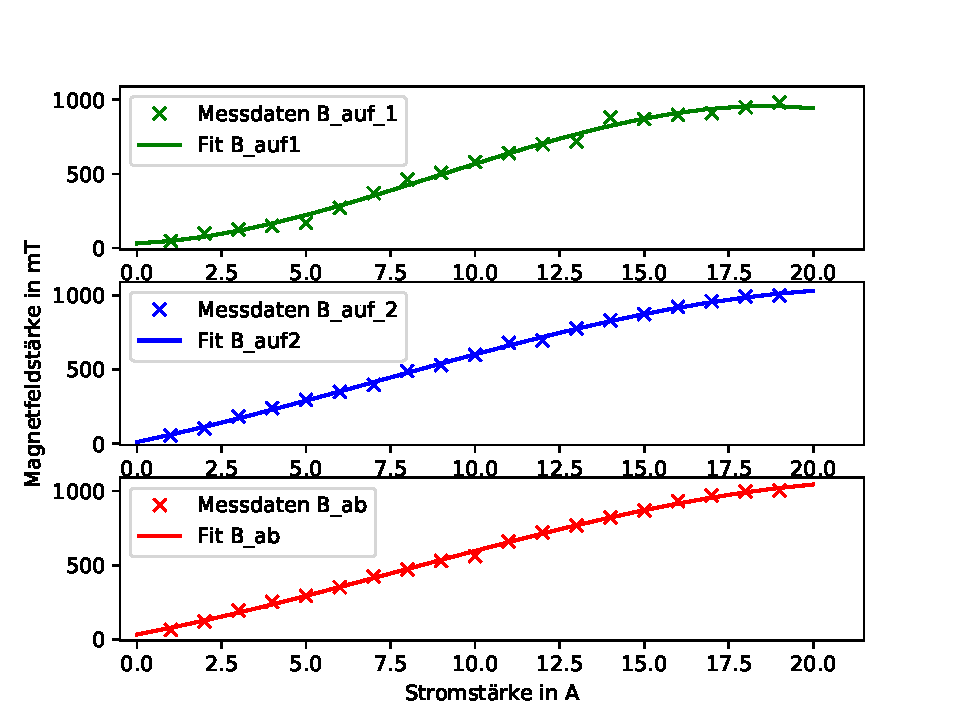
\includegraphics{Pics/Hysterese.pdf}
  \caption{Ausgleichsrechnungen f\"ur die erste steigende, die zweite steigende und die
  abfallende Hysteresekurve.}
  \label{fig:hysterese}
\end{figure}

\subsection{Spektrallinien}

Zur Auswertung der Spektrallinien werden zun\"achst die Wellenl\"angenver\"anderungen $\delta\lambda$ bestimmt:
\begin{align}
  \delta\lambda = \frac{1}{2}\frac{\delta S}{\Delta S}\Delta\lambda_D
\end{align}
Dabei steht $\delta S$ f\"ur den Abstand zwischen den aufgespaltenden Linien in Pixel und $\Delta S$ f\"ur
den Abstand zwischen den Linien ohne angelegtem Magnetfeld. Eine Verschiebung $\Delta\lambda$ in der
Wellenl\"ange ist gleichbedeutend mit einer Verschiebung $\Delta\nu$ in der Frequenz.
Es ergibt sich durch Differenzieren
f\"ur die Energiedifferenz:
\begin{align}
  \Delta E = h\cdot\Delta\nu = \frac{hc}{\lambda^2}\delta\lambda
\end{align}
Daraus folgt für den Lande-Faktor $g$:
\begin{align}
  g = \Delta E \cdot \frac{1}{\mu_BB(I)}
\end{align}

Als erstes wird die rote Spektrallinie ausgewertet. Die Dicke der Lummer-Gehrcke-Platte beträgt 4mm
und der Brechungsindex für die rote Spektrallinie liegt bei $n=\SI{1.4567}{}$. Die Wellenlänge beträgt
$\SI{643.8}{\nano\metre}$. In Abbildung \ref{fig:rotohneb} ist ein Ausschnitt der Aufnahme der roten Spektrallinie ohne
äußeres Magnetfeld dargestellt. Ausschnitte der Aufnahmen für die lineare beziehungsweise zirkulare Polarisation, bei einem
Magnetfeld von $\SI{601}{\milli\tesla}$, sind in Abbildung
\ref{fig:rotpi} und \ref{fig:rots} dargestellt.

\begin{figure}
  \centering
  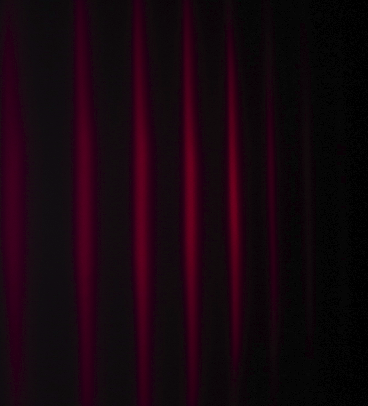
\includegraphics[width=0.6\textwidth]{Pics/rotohneb.png}
  \caption{Ein Ausschnitt der Aufnahme zur Vermessung der roten Spektrallinie ohne äußeres Magnetfeld.}
  \label{fig:rotohneb}
\end{figure}

\begin{figure}
  \centering
  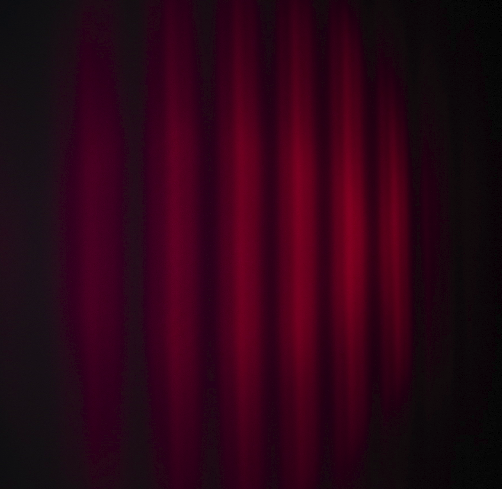
\includegraphics[width=0.6\textwidth]{Pics/rotpi.png}
  \caption{Ein Ausschnitt der Aufnahme zur Vermessung der roten Spektrallinien mit äußerem Magnetfeld und linearer Polarisation.}
  \label{fig:rotpi}
\end{figure}

\begin{figure}
  \centering
  
\includegraphics[width=0.6\textwidth]{Pics/rots.png}
  \caption{Ein Ausschnitt der Aufnahme zur Vermessung der roten Spektrallinien mit äußerem Magnetfeld und zirkularer Polarisation.}
  \label{fig:rots}
\end{figure}

Wie zu erwarten, tritt in der $\pi$-Komponente keine Aufspaltung auf. Es ergibt sich somit ein Lande-Faktor
von $g_\pi=0$. In der $\sigma$-Komponente ist dagegen eine Aufspaltung erkennbar. Die gemessenen Abstände
zwischen den Maxima für die Spektrallinie ohne Magnetfeld $\Delta S$ und die Abstände für die Spektrallinie mit Magnetfeld
und zirkularer Polarisation $\delta S$ sind in Pixel in Tabelle \ref{tab:rot} aufgelistet.
Es ergibt sich für den Lande-Faktor ein Wert von
\begin{align}
  g_\sigma = \SI{1.85(20)}{}
\end{align}

\begin{table}
  \centering
  \begin{tabular}{c c}
    \toprule
    $\Delta S$ / px & $\delta S_\sigma$ / px\\
    \midrule
        \SI{176.70}{}  &   \SI{125.83}{}\\        
        \SI{138.29}{}  &  \SI{121.24}{}\\
        \SI{115.24}{}  &  \SI{104.20}{}\\
        \SI{107.57}{}  &  \SI{106.08}{}\\
        \SI{99.88}{}  &   \SI{87.15}{}\\
        \SI{99.87}{}  &   \SI{94.72}{}\\
    \bottomrule
  \end{tabular}
  \caption{Gemessene Abstände zwischen den Maxima der roten Spektrallinie.}
  \label{tab:rot}
\end{table}

Als nächstes wird die blaue Spektrallinie ausgewertet. Der Brechungsindex beträgt $n=\SI{1.4635}{}$ und
die Wellenlänge liegt bei $\SI{480}{\nano\metre}$. Ein Ausschnitt der verwendeten Aufnahme für die Spektrallinie
ohne Magnetfeld ist in Abbildung \ref{fig:blauohneb} dargestellt. Für die Vermessung der $\sigma$-Komponente
wird ein äußeres Magnetfeld von $\SI{353}{\milli\tesla}$ erzeugt. Ein Ausschnitt der Aufnahme ist in Abbildung \ref{fig:blaus} abgebildet.
Die Aufnahme der $\pi$-Komponente erfolgte dagegen bei einem Magnetfeld von $\SI{995}{\milli\tesla}$. Die Aufnahme befindet sich in Abbildung \ref{fig:blaupi}.

\begin{figure}
  \centering
  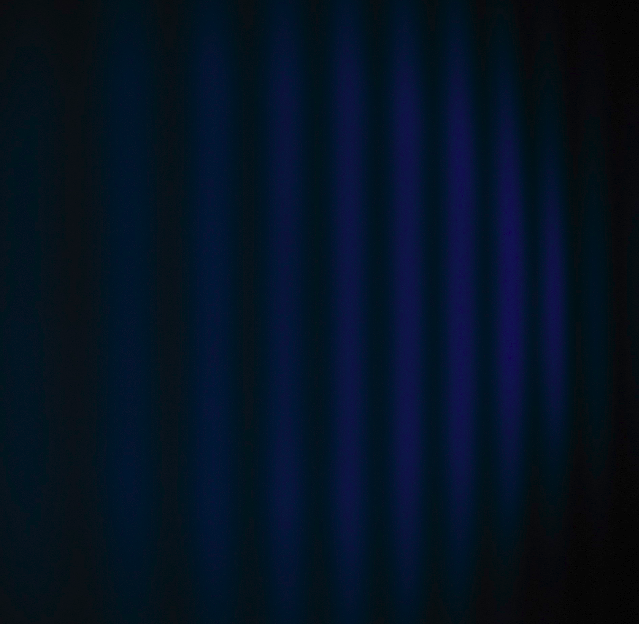
\includegraphics[width=0.6\textwidth]{Pics/blauohneb.png}
  \caption{Ein Ausschnitt der Aufnahme zur Vermessung der blauen Spektrallinie ohne äußeres Magnetfeld.}
  \label{fig:blauohneb}
\end{figure}

\begin{figure}
  \centering
  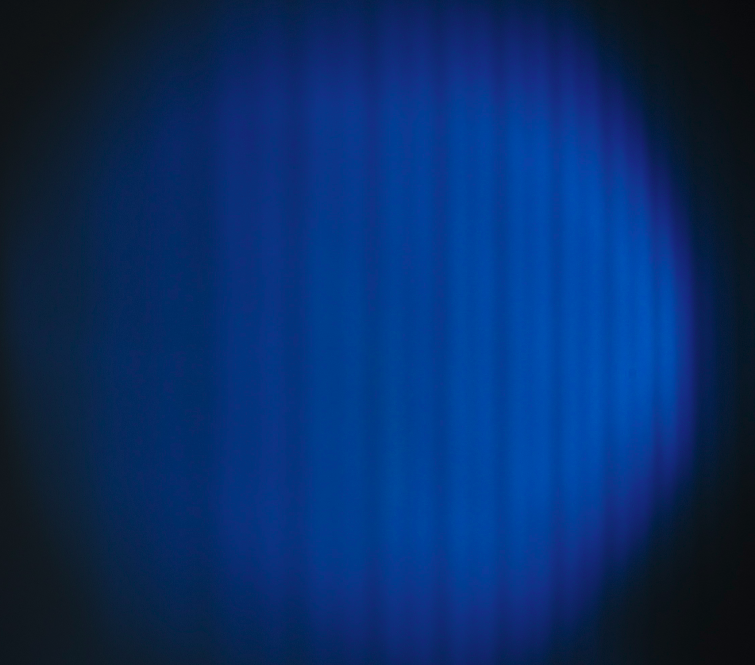
\includegraphics[width=0.6\textwidth]{Pics/blaup.png}
  \caption{Ein Ausschnitt der Aufnahme zur Vermessung der blauen Spektrallinien mit äußerem Magnetfeld und linearer Polarisation.}
  \label{fig:blaupi}
\end{figure}

\begin{figure}
  \centering
  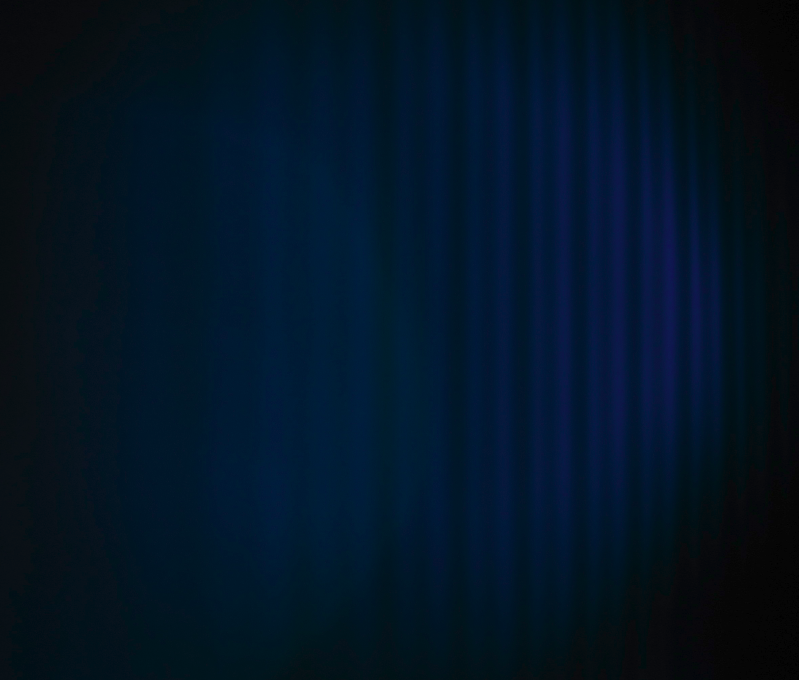
\includegraphics[width=0.6\textwidth]{Pics/blaus.png}
  \caption{Ein Ausschnitt der Aufnahme zur Vermessung der blauen Spektrallinien mit äußerem Magnetfeld und zirkularer Polarisation.}
  \label{fig:blaus}
\end{figure}

Die gemessenen Abstände in Pixel zwischen den Maxima für die verschiedenen Konfigurationen sind in Tabelle \ref{tab:blau} dargestellt.
Es ergeben sich die Lande-Faktoren:
\begin{align}
  g_\sigma &= \SI{1.9(3)}{}\\
  g_\pi    &= \SI{0.70(13)}{}
\end{align}

\begin{table}
  \centering
  \begin{tabular}{c c c}
    \toprule
    $\Delta S$ / px & $\delta S_\pi$ / px & $\delta S_\sigma$\\
    \midrule
        \SI{260.95}{}  &   \SI{130.57}{}  & \SI{110.37}{} \\        
        \SI{257.94}{}  &   \SI{118.71}{}  & \SI{110.38}{} \\
        \SI{232.72}{}  &   \SI{ 97.93}{}  & \SI{104.41}{} \\
        \SI{199.07}{}  &   \SI{118.71}{}  & \SI{101.42}{} \\
        \SI{168.22}{}   &  \SI{100.27}{}  & \SI{ 92.48}{} \\
        \SI{157.02}{}   &  \SI{ 94.96}{}  & \SI{101.43}{} \\
        \SI{151.40}{}  &   \SI{ 80.13}{}  & \SI{ 83.52}{} \\
        \SI{137.39}{}   &  \SI{ 86.06}{}  & \SI{ 83.53}{} \\
        \SI{120.56}{}   &  \SI{ 94.97}{}  & \SI{ 80.55}{} \\
    \bottomrule
  \end{tabular}
  \caption{Gemessene Abstände zwischen den Maxima der blauen Spektrallinie.}
  \label{tab:blau}
\end{table}
